


%%% Highlight dynamic sim
%%%% - new facilities wont break sim (e.g., adding non-interacting facility, adding recycle-capable reactors in a non-recycle scenario, etc.)
%%%% - flexibility
%%%% - repo accepting multiple waste forms

\section{Methodology \& Implementation}\label{sec:methods}

Dynamic Resource Exchange (DRE) is a inter-simulation, optimization-based
methodology for determining transactions between suppliers and consumers. The
core solution strategy is agnostic to resource types. The DRE is designed to
support fuel cycle simulation, which is highly dependent on specific resource
properties (material isotopic vectors), through its agent communication
framework. Because the communication framework can be specialized to any
abstract resource type, the methodology and framework can be adapted to other
complex supply chains.

The DRE enables the constrained transaction of complex resources between
entities in a simulation given a measure of cardinal preference for each
potential transactions. The full formulation of the description of supply and
demand in the fuel-cycle context is denoted the Nuclear Fuel Cycle
Transportation Problem (NFCTP), a variant of the classic family of
transportation problems in optimization. Suppliers and consumers provide
information about their supply and demand during an initial information
gathering phase. Complex constraints can be supplied during this phase. Supply
and demand is then translated into a resource-agnostic \textit{Exchange
  Graph}. The graph can be solved feasibly with a heuristic or optimally by
translating it into a mixed integer-linear program. Given a solution, final
trades are constructed and executed. In order to provide a more concrete
discussion, all descriptions of the DRE and its mechanisms assume an
material-based exchange, as one would normally find in a fuel-cycle simulation
context.

\Secref{meth:mtp} begins by providing a short overview of the
classic optimization tools on which this work is built. An outline of the DRE
methodology's progression with respect to the simulation architecture is
described in \secref{meth:comm}. \Secref{abm:dre:info} then details the
interface that agents within the simulation have with the DRE in order to
communicate supply and demand information. A description of the DRE's
graph-based and formulation based definitions and solution techniques is
provided in \secref{abm:dre:fctp}. Finally, \secref{meth:tariff} describes a new
\texttt{Region} archetype in the \Cyclus ecosystem that utilizes the DRE to
enable the \textit{in situ} modeling of inter-state trade instruments, such as
tariffs.

This section represents the culmination of significant previous effort
\cite{gidden_agent-based_2013, gidden_agent-based_2014,
  gidden_agent-based_slc_2013}. What follows constitutes the refinement of
previous descriptions of the DRE methodology with lessons learned from initial
implementation and usage.

\subsection{Multicommodity Transportation Problems}\label{meth:mtp}

Supply and demand in a nuclear fuel cycle context is inherently a multicommodity
problem: a light water reactor can be fueled by both UOX and MOX fuel, for
instance. How it is fueled is a result both of fuel availability and associated
preferences. In order to allow for complex physical and chemical constraints on
both processes and inventories, an optimization-based approach is used which
employs economics-based proxies to arrive at a solution of resource transfers
within a simulation time-step.

The DRE translates agent supply and demand into a version of the Multi-commodity
Transportation Problem (MTP) \cite{even1975complexity} which belongs to the
network flow family of optimization problems. A network flow problem is
represented by a graph, $G(N, A)$, comprised of nodes $N$ and arcs $A$. If flow
can occur between some node $i$ and some other node $j$, then it flows along arc
$(i, j)$. Given a graph instance, optimal flow between nodes can be found
provided \textit{objective coefficients} and
\textit{constraints}. \textit{Decision variables} for this optimization problem
comprise the optimal \textit{flow assignment}. If all decision variables are
linear, then the resulting formulation is termed a Linear Program (LP). If some
decision variables are integer (e.g., binary), the formulation is termed a
Mixed-Integer Linear Program (MILP).

Transportation problems model the flow of a commodity between source nodes and
sink nodes which can have supply and demand constraints. A more complex
transportation-problem formulation can support systems in which supply or demand
can be met by multiple commodities.  There is a unit cost $c_{i,j}^{h}$ for
commodity $h$ to traverse arc $(i,j)$. A supplier of commodity $h$ has a certain
supply capacity $s_i^h$ which cannot be surpassed and consumers of commodity $h$
have a certain demand level which must be met, $d_i^h$.

In the simplest extension from the single-commodity to multi-commodity
transportation problem, arc constraints for all commodities are combined, i.e.,
there is a single capacity $u_{i,j}$ for a given arc $(i, j)$. A classic
application of this enhanced complexity deals with data networks. Multiple
classifications of data exist, but they all must traverse the same network
infrastructure. Accordingly, the infrastructure can only accommodate a certain
quantity of total flow among all communication types. The formulation of the
multi-commodity flow problem is shown in Equation \ref{eqs:MCTP}. Note the
commodity coupling in Equation \ref{eqs:MCTP_cap}.

%%% 
\begin{subequations}\label{eqs:MCTP}
  \begin{align}
    %%
    \min_{x} \:\: & 
    \sum_{i \in I}\sum_{j \in J}\sum_{h \in H} c_{i,j}^{h} x_{i,j}^{h}
    & \label{eqs:MCTP_obj} \\
    %%
    \text{s.t.} \:\: &
    \sum_{j \in J} x_{i,j}^{h} \leq s_{i}^{h}
    &
    \forall \: i \in I, \forall \: h \in H \label{eqs:MCTP_sup} \\
    %%
    &
    \sum_{i \in I} x_{i,j}^{h} \geq d_{j}^{h}
    & 
    \forall \: j \in J, \forall \: h \in H \label{eqs:MCTP_dem} \\
    %%
    &
    \sum_{h \in H} x_{i,j}^{h} \leq u_{i,j}
    & 
    \forall \: (i, j) \in A \label{eqs:MCTP_cap} \\
    %%
    &
    x_{i,j}^{k} \geq 0
    &
    \forall \: (i, j) \in A, \forall \: h \in H \label{eqs:MCTP_x}
    %%
  \end{align}
\end{subequations}
%%% 

The proceeding sections describe how agent state at a given point in time in a
simulation is translated into constraint and cost parameters (e.g., $s$, $d$,
and $c$ in Equation \ref{eqs:MCTP}). While the DRE-based formulation is not a
direct mirror of Equation \ref{eqs:MCTP}, it is a useful basis of
comparison. Arcs in the DRE-based formulation are identified by their commodity
and grouped into appropriate constraints, whereas the multicommodity nature
arises in Equation \ref{eqs:MCTP_cap} as a constraint on individual arcs.

\subsection{Communication between Simulation and Formulation}\label{meth:comm}

Defining a robust interface for the communication between simulation and
optimization components is one of the most difficult aspects in constructing a
single, combined framework. A clear mapping of simulation and agent concepts to
formulation coefficients, constraints, and parameters is required. Conceptually,
the DRE implements this interface in three layers as shown in Figure
\ref{fig:dre_impl}.

\begin{figure}
  \begin{center}
    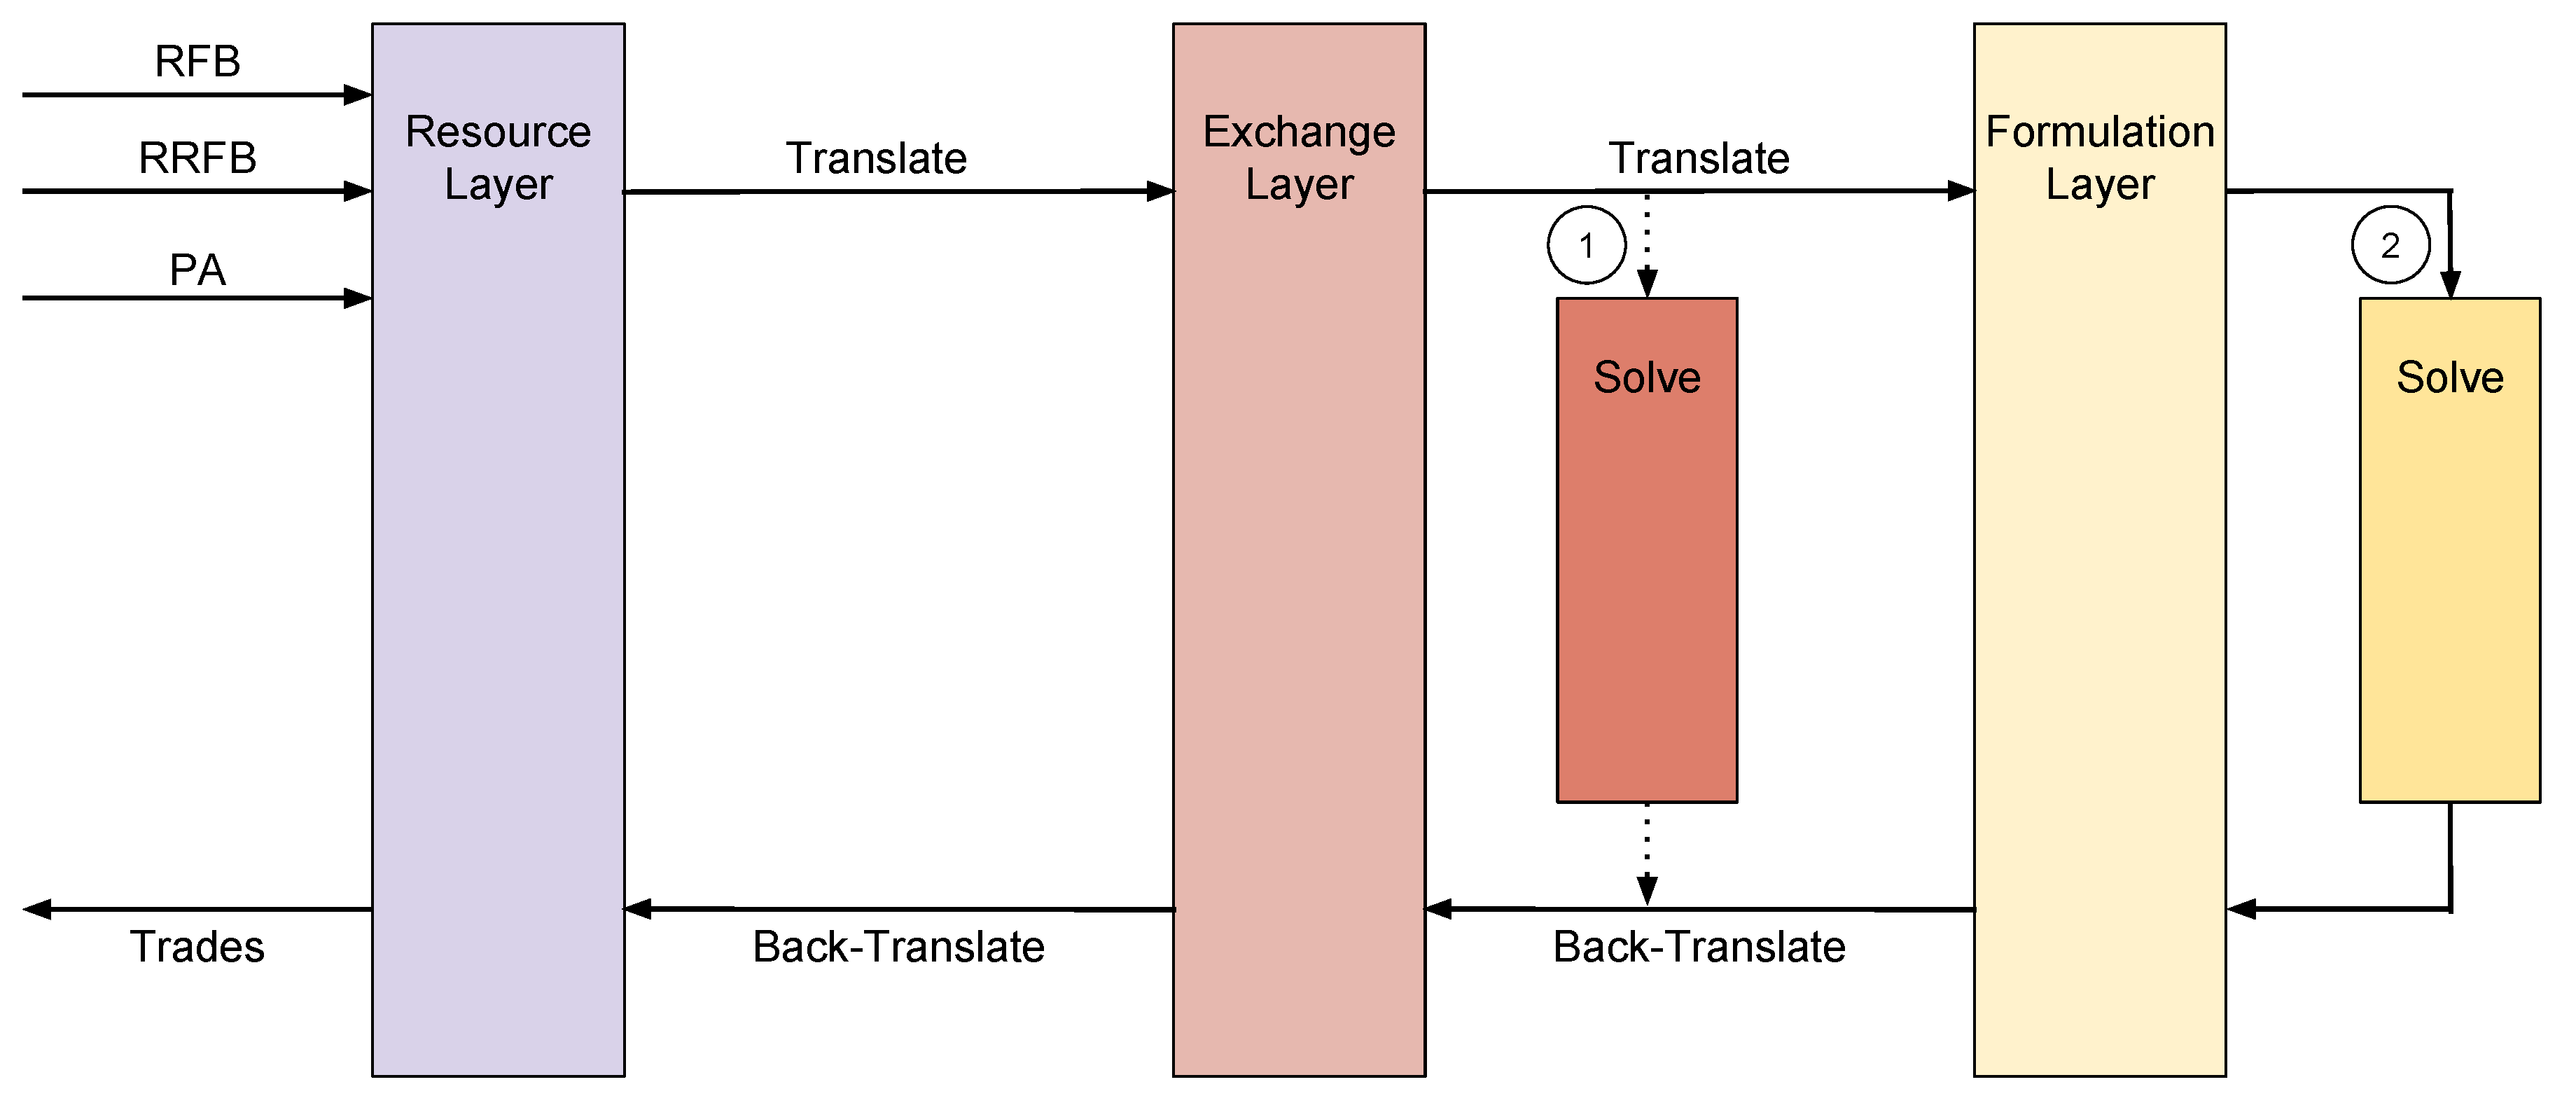
\includegraphics[width=\textwidth]{exchange_xlation.pdf}
    \caption[]{
      \label{fig:dre_impl}
      The full DRE workflow is shown. The information gathering phase, described
      in \secref{abm:dre:info}, results in the resource layer. The resource
      layer is translated to the exchange layer; marked by the number $1$, a
      decision is made whether to continue translation or to directly solve the
      instance, as described in \secref{abm:dre:nfctp:heur}. If the exchange is
      not solved, it is translated into an instance of the NFCTP resulting in
      the formulation layer as shown in \secref{abm:dre:milp}. A choice of
      solver is made, marked by the number $2$, and the instance is solved.  The
      solution is back-translated through the exchange and resource layers. The
      result is a series of resource trades to be executed in the simulation.}
  \end{center}
\end{figure}

The first layer includes information for specific
\code{Resource} \footnote{Terms that directly map to names of C++ classes in the
  \Cyclus code base are formatted as shown for clarity.} types. For example, a
\code{Material}-based exchange is used for agents to communicate supply and
demand information regarding \code{Material} objects. The \textit{resource
  layer} is the point of entry and exit of the DRE framework. It is the
agent-facing interface of the DRE: supply and demand is provided to the DRE as
input during the information gathering step, and trades to be executed are
provided to agents as output.

The second layer, called the \textit{exchange layer}, is a
\code{Resource}-agnostic representation of supply and demand. Supply/demand
constructs in the first layer are translated into stateful objects representing
nodes, arcs, constructs that carry constraint information, \textit{et
  cetera}. The collection of objects and structures combine to create an
\code{ExchangeGraph}. Any custom, \Cyclus-aware solver can be applied to an
\code{ExchangeGraph} to determine a feasible solution to the DRE.

In order to use sophisticated, 3\textsuperscript{rd} party LP and MILP solving
libraries, the \code{ExchangeGraph} must be translated into an appropriate data
structure representing an instance of the NFCTP, resulting in the
\textit{formulation layer}. The Open Solver Interface (OSI) \cite{coinosi} is
used to create the necessary formulation structures, including a constraint
matrix and objective coefficient vector. The NFCTP instance is then solved.

After a feasible, perhaps optimal, solution to the NFCTP is found, whether in
the exchange or formulation layer, the solution is back-translated to the
resource layer. The agents associated with successful supply-demand connections
are informed, and trades of resources between agents are executed.

\subsection{Agent Interaction with the DRE}\label{abm:dre:info}

\subsubsection{Supply and Demand}

The DRE begins with three \textit{phases}, the terminology of which is
influenced from previous supply chain agent-based modeling work
\cite{julka_agent-based_2002}. Importantly, this information-gathering step is
agnostic as to the supply-demand matching algorithm used, it is concerned only
with querying the current status of supply and demand in the simulation. The
collective information gathering procedure is shown in Figure
\ref{fig:procedure}.

\begin{figure}
  \centering
  \makebox[\textwidth][c]{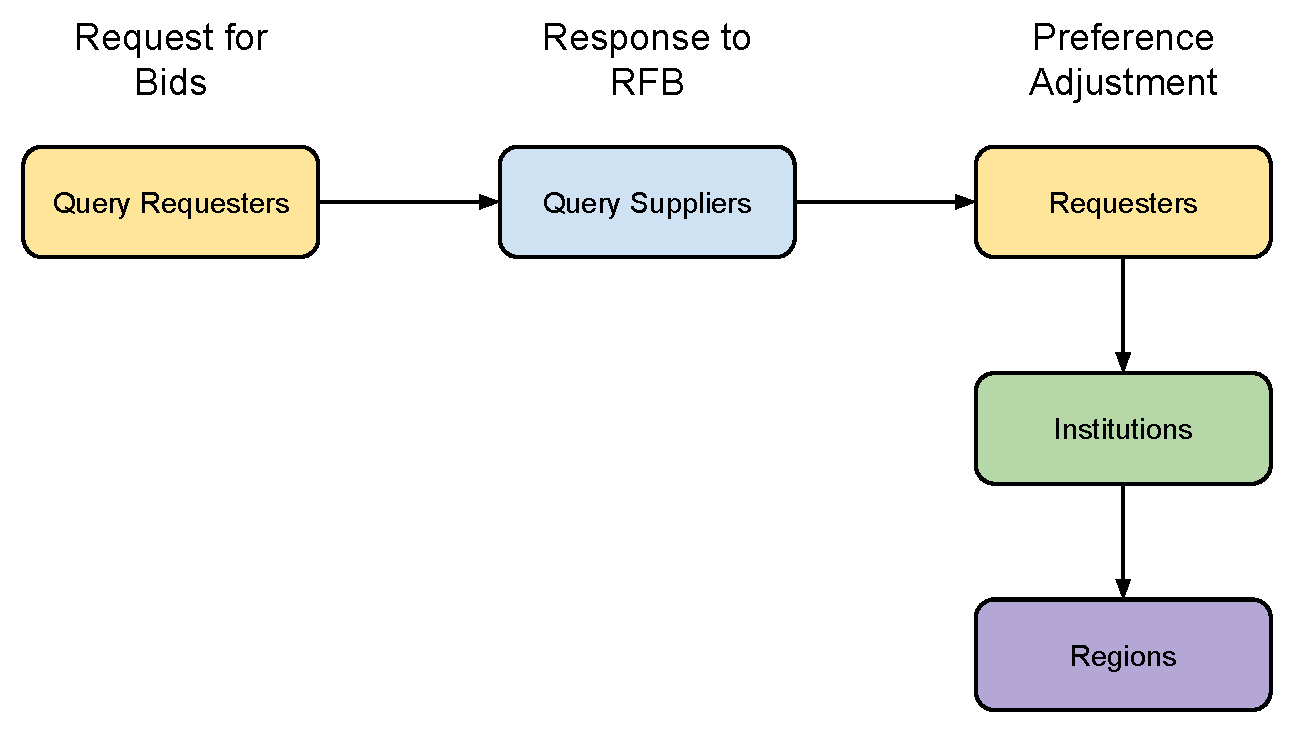
\includegraphics[width=0.8\textwidth]{info_gathering_phases.pdf}}
  \caption[]{Schematic illustrating the DRE's information
    gathering phases: Request for Bids (RFB), Response to Request for Bids
    (RRFB), and Preference Adjustment (PA).\label{fig:procedure}}
\end{figure}

The first phase allows consumers of commodities to denote both the quantity of a
commodity they need to consume as well as the target isotopics, or quality, by
\textit{posting} their demand to the market exchange. This posting informs
producers of commodities what is needed by consumers, and is termed the
\textit{Request for Bids} (RFB) phase. Consumers are allowed to over-post, i.e.,
request more quantity than they can actually consume, as long as a corresponding
capacity constraint accompanies this posting. Requests can be denoted as
\textit{exclusive}. An exclusive request is one that must either be met in full
or not at all. Exclusive requests allow the modeling of quantized, packaged
transfers, e.g., fuel assemblies. 

Consumers are allowed to post demand for multiple commodities that may serve to
meet the same capacity, and the collection of all commodities requested is
termed its \textit{request portfolio}. For example, consider an LWR that can be
filled with MOX or UOX. It can post a demand for both, but must define a
preference over the set of possible commodities that can be consumed. Such
requests are termed \textit{mutual requests}. Another example is that of an
advanced fuel fabrication facility, i.e., one that fabricates fuel partially
from separated material that has already passed through a reactor. Such a
facility can choose to fill the remaining space in a certain assembly with
various types of fertile material, including depleted uranium from enrichment or
reprocessed uranium from separations. Accordingly, it could demand both
commodities as long as it provides a corresponding constraint with respect to
total consumption. A set of exclusive requests may also be grouped as mutual
requests, in which case the set is termed \textit{mutually exclusive}.

At the completion of the RFB phase, the market exchange will have a set of
request portfolios. Each portfolio consists of a set requests. Arbitrary
constraints over the set of requests can be provided that are functions of
quantity, $x$, or quality, $q$.  When communicating constraining information,
agents must provide a total constraining quantity, $b$, and a \textit{constraint
  coefficient conversion function}, $\beta (q_{i, j})$. Utilizing this
information, constraints similar to Equation \ref{eqs:MCTP_dem} can be
constructed for all possible trades $A_j$ for requester $j$,

\begin{equation}\label{meth:constr}
  \sum_{(i, j) \in A_j} \beta (q_{i,j}) x_{i, j} \geq b.
\end{equation}

\noindent
Each request additionally has an associated preference. For requests that
mutually satisfy a given demand, a preference distribution over those requests
informs the solver as to which should be satisfied first, given the
constraints. Finally, each request portfolio has a specific quantity associated
with it.

The second phase allows suppliers to \textit{respond} to the set of request
portfolios, and is termed the \textit{Response to Request for Bids} (RRFB) phase
(analogous to Julka's Reply to Request for Quote phase
\cite{julka_agent-based_2002}). Each request portfolio comprises requests
for some set of commodities. Accordingly, for each request, suppliers of that
commodity denote production capacities and an isotopic profile of the commodity
they can provide. Suppliers are allowed to offer the null set of isotopics as
their profile, effectively providing no information. Suppliers are also allowed
to denote responses as exclusive, as is done in the RFB phase. Supply responses
can also be grouped into mutual responses, and sets of responses may be mutually
exclusive. This functionality again supports the notion of quantized orders,
e.g., in the case of fuel assemblies. The full collection of responses for a
given supplier is denoted as its \textit{supply portfolio}.

A supplier may have its production constrained by communicating the same
information as consumers. Constraints corresponding to Equation
\ref{eqs:MCTP_sup} are constructed in the same manner as Equation
\ref{meth:constr}. Suppliers can provide one or more constraints. For example, a
processing facility may have both a throughput constraint (i.e., it can only
process material at a certain rate) and an inventory constraint (i.e., it can
only hold some total material). Further, the facility could have a constraint on
the quality of material to be processed, e.g., it may be able to handle a
maximum radiotoxicity for any given time step which is a function of both the
quantity of material in processes and the isotopic content of that
material. Multiple of such constraints are allowed. At the completion of the
RRFB phase the possible connections between supplier and producer facilities,
i.e., the arcs in the graph of the transportation problem, have been established
with specific capacity constraints defined both by the quantity and quality of
commodities that will traverse the arcs.

\subsubsection{Preferences}

The final phase of the information gathering procedure allows consumer
facilities to adjust their set of preferences and for managers of consumer
facilities to affect the consumer's set of preferences. Accordingly, the last
phase is termed the \textit{Preference Adjustment} (PA) phase. By allowing
facility managers, i.e., a facility's institution and region, to also adjust
preferences, socio-economic models are allowed to inform the exchange of
resources. For example, a region can detect a trans-regional trade between one of
its facilities and a facility in another region. If a tariff model is employed,
the trade preference and be diminished or even removed.

For facilities, preference adjustment provides a mechanism to act with arbitrary
complexity in response to offers provided by producer facilities. Consider the
example of a reactor facility that requests two fuel types, MOX and UOX, and
receives two responses to its request for MOX, each with different isotopic
profiles. It can then assign preference values over the set of potential MOX
providers. Repositories provide another prime example where preference
adjustment can be naturally employed. A repository may have a defined preference
of material to accept based upon its heat load or radiotoxicity, both of which
are functions of the quality, or isotopics, of a material. In certain
simulators, limits on fuel entering a repository are imposed based upon the
amount of time that has elapsed since the fuel has exited a reactor, which can
be assessed during this phase. The time constraint is, in actuality, a
constraint on heat load or radiotoxicity (one must let enough of the fission
products decay). A repository could analyze possible input fuel isotopics and
set the arc preference of any that violate a given rule to 0, thereby
eliminating that arc.

The game theoretic notion of preferences can be quite useful in fuel cycle
simulation. Specifically, cardinal utility, or cardinal preferences
\cite{strotz_cardinal_1953} provides a relative measure of preference such that
any two preferences can be directly compared, provided an arbitrary scaling,
similar to the comparison of costs in a system. The notion of preference also
nicely extends the work of Oliver's affinity metric
\cite{oliver_geniusv2:_2009}. Additionally, costs in a nuclear fuel cycle
simulation have reasonably large uncertainty \cite{shropshire_advanced_2009} and
are generally applied to the output of a simulator as a post-processing
step. Therefore, preferences, a proxy of cost, can be used to drive consistent
decision-making within a simulation.

There exists a body of literature that examine Nash Equilibria in the context of
optimal flow models
\cite{mazumdar_fairness_1991,nagurney_supply_2002,song_nash_2002}. However, the
complexity of such models quickly brings them out of the scope of the needs for
dynamic modeling of multi-lateral scenarios ranging 100+ years in a
``reasonable'' amount of computation time.

\subsubsection{Trades}

The information gathering phase defines the population of \textit{potential}
trades. The system is then solved by either a heuristic or optimization solver,
resulting in a feasible set of \textit{finalized} trades. The DRE is completed
at a given time step when trades are \textit{executed} by instructing all
supplier agents to send their finalized trades to consumer agents.

\subsection{The Nuclear Fuel Cycle Transportation Problem}\label{abm:dre:fctp}

An instance of supply and demand defined by the DRE's information gathering step
is cast to a constrained, bipartite network which represents a variant of the
MTP, entitled the \textit{Nuclear Fuel Cycle Transportation Problem} (NFCTP). It
can be solved by any heuristic that provides a feasible solution to such
networks are valid.  For this work, a greedy heuristic is designed and
implemented. The system can be solved optimally, however, by formulating the
system as a mathematical program, and a MILP formulation is provided
provided. Formulated as a MILP, the system can be solved with any available
solver. \cbc\cite{forrestcbc}, a popular open-source branch-and-bound solver, is
used in this work.

\subsubsection{Exchange Graph}

Objects and data structures generated in the information gathering procedure are
used in the formal definition of the NFCTP by mapping the agent-supplied
information onto a \textit{bipartite} graph. This mapping allows for the
translation from the resource to exchange layers shown in Figure
\ref{fig:dre_impl}. Information is mapped to properties of arcs, which represent
proposed trades, and portfolio-based node groupings. The components of an
Exchange Graph have a one-to-one mapping with simulation entities. For example,
nodes in the graph represent distinct bids and requests provided by agents.

Each supply and request portfolio can be considered separately, i.e., there is
no information shared between two portfolios of a given agent. The set of supply
portfolios is denoted as $S$ and the set of request portfolios is denoted as
$R$; each agent may have multiple portfolios in a given exchange. Each
supply portfolio is comprised of $s_M$ supply nodes, and each request portfolio
is comprised of $r_N$ nodes. For notation simplicity, nodes within portfolios
are referred to with single indices (e.g., $i$ or $j$), and collections of arcs
(connections between supply and request nodes) associated with a given portfolio
are referred to as $(i, j) \in A_s$ and $(i, j) \in A_r$, for supply and request
portfolios respectively.

For each request node, $j$, there may be many bid nodes; however, there is a
one-to-one mapping between bid nodes and request nodes. In other words, a given
bid node, $i$, is a unique response to a request node, $j$. Because of defined
constraints, there may not be sufficient supply in the simulated exchange. To
ensure a feasible solution, an unconstrained false supply node is added to the
Exchange Graph. Additionally, false nodes are added to each request portfolio
and are connected to the false supply source. These arcs are denoted as
\textit{false arcs}. Figure \ref{fig:ex_false} shows a fully defined Exchange
Graph. As an example, $A_s$ in this example is defined as 
$\left \{ (i, j), (i', j') \right \}$.

\begin{figure}
  \begin{center}
    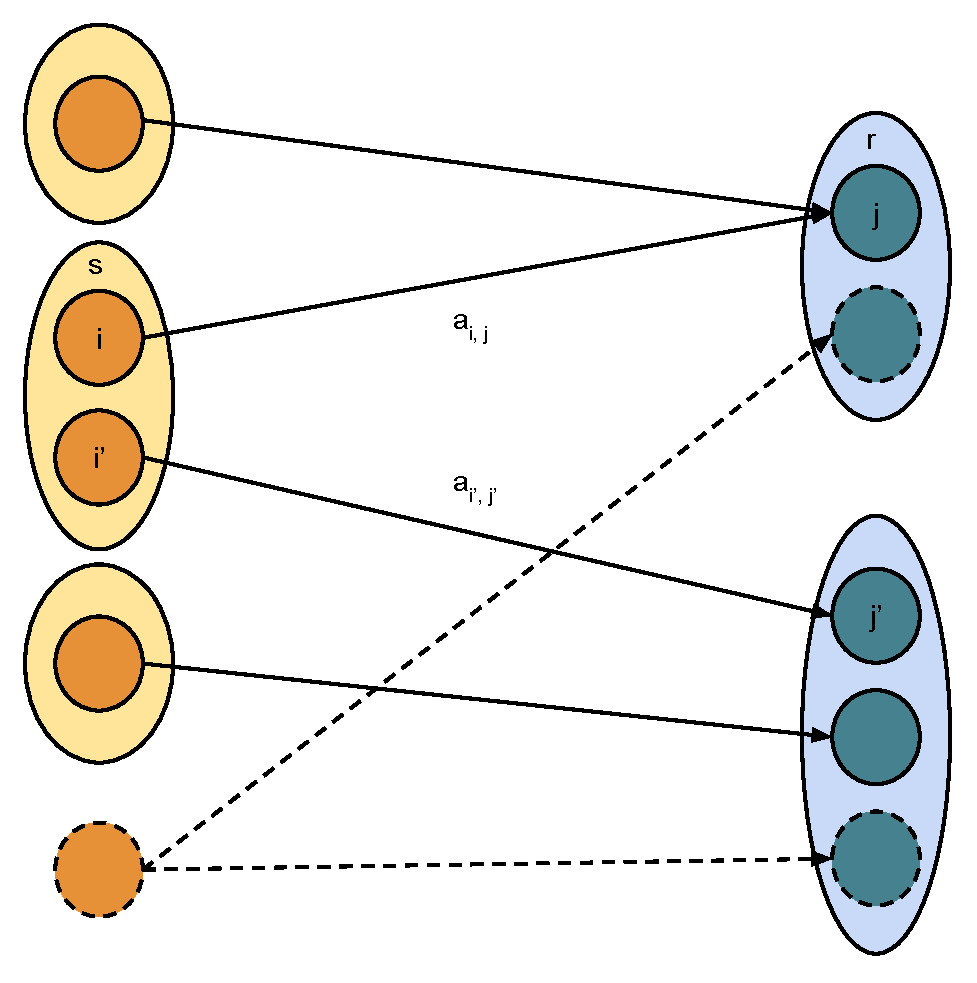
\includegraphics[width=0.75\textwidth]{exchange_false_notated.pdf}
    \caption{An example exchange with supply nodes colored orange on left
      and request nodes colored blue on right. As shown, there can be multiple
      supply nodes connected to a request node, but each supply node corresponds
      uniquely to one request node. It is a specific response to that request,
      as outlined in the RRFB phase. In this example, there are three
      supplier agents and two consumer agents. The second consumer has two
      requests (for different commodities) which may satisfy its demand. The
      second supplier can supply the commodities requested by both consumers and
      has provided two bids accordingly. The false supplier and consumer nodes are
      shown with a dashed outline. Similarly, false arcs are dashed. Note that
      the false nodes have no associated portfolio structure -- there are no
      constraints associated with false nodes and arcs. The inclusion of a false
      supplier and consumer guarantees a feasible solution.}
    \label{fig:ex_false}
  \end{center}
\end{figure}

In the bipartite graph, portfolios act as partitions that group nodes together.
Each portfolio has a set of commodities, $H$, associated with it. These are
denoted $H_s$ for supply portfolios and $H_r$ for request portfolios. Node
groups share a set of common constraints, $K$, and request node groups share a
common notion of satisfiable quantity, i.e., a default mass-based
constraint. Each constraint has a constraining value, $b_s^k$ and $b_r^k$,
respectively.

Additionally, each portfolio and constraint has a defined constraint coefficient
conversion function, denoted $\beta_s^k$ for supply portfolios and $\beta_r^k$
for request portfolios. Request portfolios are provided a mass constraint by
default for which coefficients are unity and whose constraining value is is
$b^{x}_{r}$. If requested commodities are labeled as \textit{mutual}, then a
weighting coefficient is generated for each request in the mutual set, $M$, in
order to support cases where different commodities are requested with different
quantities. The coefficient is defined by the ratio between the the average
request quantity over all mutual requests and $x_m$

\begin{equation}\label{meth:mutual-coeff}
  \beta_{r, m} = \frac{\overline{x_M}}{x_m},
\end{equation}

The constraint conversion functions are utilized in the NFCTP by applying them
to the proposed resource transfers, creating constraint
coefficients. Coefficients for supply constraints are defined as

\begin{equation}
  a^k_{i, j} = \beta_s^k(q_{i,j}).
\end{equation}

\noindent
Coefficients for request constraints are defined as

\begin{equation}
  a^k_{j, i} = \beta_r^k(q_{i,j}).
\end{equation}

Finally, for each supply-request node pair, there is an associated preference,
$p_{i, j}$. The set of all preferences is denoted $P$. Similarly, flow between a
node pair is denoted $x_{i, j}$, and the set of all flows is denoted $X$. The
possible flow on an arc is provided an upper bound by the request node quantity,
$\widetilde{x_j}$.

%\paragraph{Preferences \& Costs}

In any network flow problem, the objective coefficients associated with
transporting commodities drive the solution. Given the nature of supply and
demand constraints, the transportation problem naturally lends itself to a
minimum cost formulation. A preference-based formulation has been presented thus
far due to the difficulties of employing reasonable cost coefficients. While
directly using costs should be available to users, in practice using a more
abstract notion of preferences is simpler.

Formally, a preference function, $p_{i, j}(h)$, is defined which is a cardinal
preference ordering over a consumer's satisfying commodity set.
 
\begin{equation}
p_{i, j}(h) \:\: \forall i \in I  \:\: \forall h \in H_{r} 
\end{equation}

\noindent
A preference is assigned to each arc in the NFCTP and is a function both of the
consumer, $j$, and producer, $i$, and the quality, $q_{i, j}$, of the proposed
resource transfer from consumer to producer. The dependence on producer
encapsulates the relationship effects due to managerial preferences. The
preference set used in the NFCTP formulation follows directly from the
Preference Adjustment phase described in \secref{abm:dre:info}. A cost
translation function, $f$, is defined that operates on the commodity preference
function to produce an appropriate cost for the NFCTP.

\begin{equation}
f : p_{i,j}(h) \to c_{i,j}
\end{equation}

\noindent
For the purposes of this work, any operator that preserves preference
monotonicity and cardinal ordering is suitable.  The inversion operator has been
chosen because it preserves required features and also allows for easy
translation from preference to cost as well as translation from cost to
preference.

\begin{equation}
f(x) = \frac{1}{x}
\end{equation}

The preferences given to each false arc, $p_f$, is defined to be lower than the
lowest preference in the system, $P$.

\begin{equation}\label{eqn:falsepref}
  p_{f} < \min P
\end{equation}

Because preferences are defined as in Equation \ref{eqn:falsepref}, any false
arc will only be engaged if no other possible arc can be engage, due to capacity
constraints. If any flow is assigned to false arcs after the Exchange Graph is
solved, that flow is ignored when initiating transactions.

If cost data and a valid cost assignment methodology is developed in the future,
costs may be used directly, and the preference-to-cost translation may be
ignored.

\subsubsection{An Example Exchange Graph}

During the information gathering step in \secref{abm:dre:info}, consumers and
suppliers are queried based on \textit{commodities}. A consumer is allowed to
request multiple commodities, and a supplier is allowed to supply multiple
commodities. However, each possible resource transfer, i.e., each arc, is based
on a single commodity. Accordingly, it is possible to color each arc, given a
commodity-to-color mapping.

For example, consider the Exchange Graph shown in Figure \ref{fig:ex_groups_color}
with two fuel commodities ($A$, $B$), two requesters ($R_1$, $R_2$), and three
suppliers ($S_1$, $S_2$, $S_3$) in the configuration described by Tables
\ref{tbl:ex_sup} and \ref{tbl:ex_req}. The resulting Exchange Graph can be
colored as shown in Figure \ref{fig:ex_groups_color}.

\begin{table}[h]
\centering
\begin{tabular}{c|c}
Supplier & Commodities \\ \hline
$S_1$             & $A$         \\
$S_2$             & $A$, $B$    \\
$S_3$             & $B$         \\
\end{tabular}
\caption{A mapping from suppliers to commodities supplied.}
\label{tbl:ex_sup}
\end{table}

\begin{table}[h]
\centering
\begin{tabular}{c|c}
Consumer & Commodities \\ \hline
$R_1$             & $A$         \\
$R_2$             & $B$        
\end{tabular}
\caption{A mapping from requesters to commodities requested.}
\label{tbl:ex_req}
\end{table}

\begin{figure}
  \begin{center}
    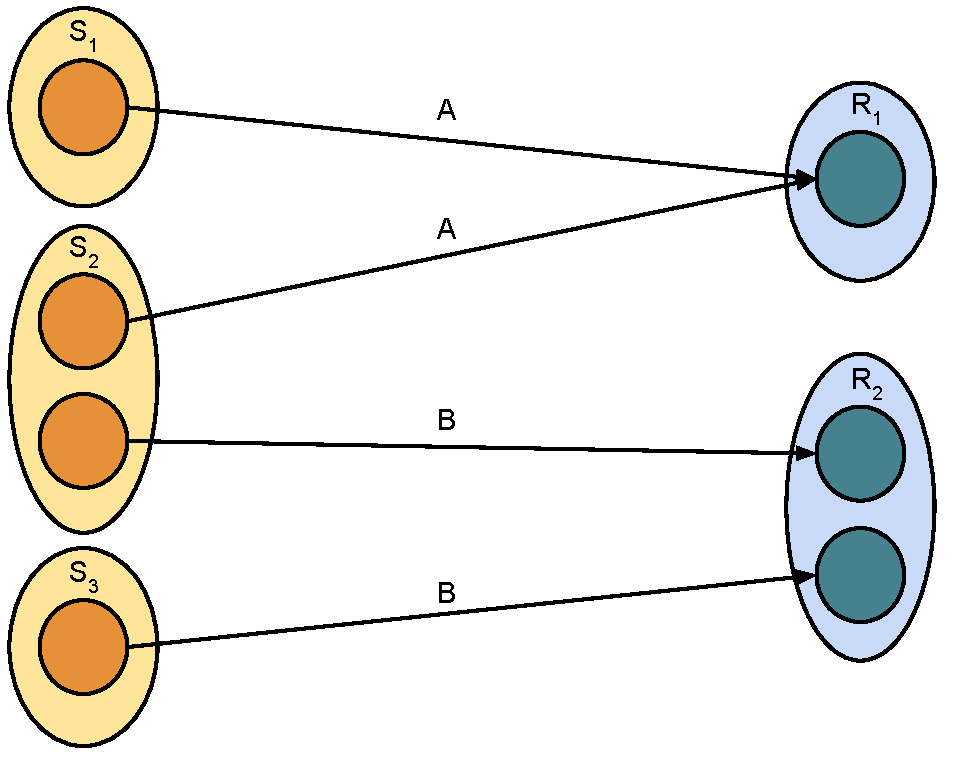
\includegraphics[width=0.75\textwidth]{exchange_groups_color.pdf}
    \caption{The same exchange shown in Figure \ref{fig:ex_false} with arcs and
      portfolios labeled based on Tables \ref{tbl:ex_sup} and
      \ref{tbl:ex_req}. }
    \label{fig:ex_groups_color}
  \end{center}
\end{figure}

The notion of commodities is critical during the information gathering step as
it is the basic classification used in communicating supply and demand. It is
also useful when an Exchange Graph is formed, because the graph may be able to
be partitioned by collections of commodities. However, once minimally connected
Exchange Graphs are established, solution mechanisms do not employ the notion of
commodities. Rather, quantities, constraints, and preferences are used.

\subsubsection{Communicating Constraints}

Constraint coefficients are determined for an arc based on the proposed resource
to be transferred along that arc, the requester's constraint conversion
functions, and the suppliers constraint conversion function. Consider a supplier
enrichment facility, $s$, which produces the commodity enriched uranium
(EU). This facility has two constraints on its operation for any given time
period: the amount of Separative Work Units (SWU) that it can process,
$b_{s}^{\text{SWU}}$, and the total natural uranium (NU) feed it has on hand.,
$b_{s}^{\text{NU}}$.  Note that neither of these capacities are measure directly in the
units of the commodity it produces, i.e., kilograms of EU. The constraint set
for $s$ is then
 
\begin{equation}\label{eqs:enr-constr-commods}
  K_{s} = \{ \text{\text{SWU}}, \text{\text{NU}} \}.
\end{equation}


Consider a set of requests for enriched uranium that this facility can possibly
meet. Such requests have, in general, two parameters: $P_{j}$, the total product
quantity (in kilograms), and $\varepsilon_{j}$, the product enrichment (in w/o
\nucl{235}{U}).\footnote{The notation for enrichment, $\varepsilon_{j}$, is
  chosen over its normal form, $x_p$, to limit confusion with the notation of
  material flow, $x_{i,j}$.}  For the purposes of this constraint set, the
quality of material in question is its enrichment, i.e.,

\begin{equation}\label{eqs:enr-q-swu}
  q_{j} \equiv \varepsilon_{j}.
\end{equation}

These values are set during the information-gathering phase of the overall
matching algorithm, and can therefore be considered constant. Further, note
that, in general, an enrichment facility's operation, or rather its capacity, is
governed by two parameters: $\varepsilon_{f}$, the fraction of \nucl{235}{U} in
its feed material, and $\varepsilon_{t}$, the fraction of \nucl{235}{U} in its
tails material. These parameters determine the amount of SWU required to produce
some amount of enriched uranium, shown in Equation \ref{eqs:swu} as well as the
amount of natural uranium, or feed, required, as shown in Equation \ref{eqs:nu}.

\begin{align}
\begin{split}
\label{eqs:swu}
SWU = & \:\: P ( V(\varepsilon_{j}) 
      + \frac{\varepsilon_{j} - \varepsilon_{f}}
               {\varepsilon_{f} - \varepsilon_{t}} V(\varepsilon_{t}) \\
      & - \frac{\varepsilon_{j} - \varepsilon_{t}}
               {\varepsilon_{f} - \varepsilon_{t}} V(\varepsilon_{f}) )
\end{split}
\end{align}

\begin{equation}
\label{eqs:nu}
F = P \frac{\varepsilon_{j} - \varepsilon_{t}}
           {\varepsilon_{f} - \varepsilon_{t}}
\end{equation}

\noindent
$P$ in Equations \ref{eqs:swu} and \ref{eqs:nu} is the amount of produced
enriched uranium, $F$ is the amount of feed, or natural uranium, and $V(x)$ is
the value function,

\begin{equation}\label{eqs:value}
  V(x) = (1-2x) \ln \left(\frac{1-x}{x}\right)
\end{equation}

Utilizing the above equations, one can denote the functional forms of the
arguments of this facility's two capacity constraints.

\begin{align}
\label{eqs:enr-prod-beta}
\beta_{s}^{\text{NU}}(\varepsilon_{j}) = & \:\: \frac{\varepsilon_{j} - \varepsilon_{t}}
                                      {\varepsilon_{f} - \varepsilon_{t}} \\
\begin{split}
\label{eqs:enr-swu-beta}
\beta_{s}^{\text{SWU}}(\varepsilon_{j}) = & \:\: V(\varepsilon_{j}) \\
                         & + \frac{\varepsilon_{j} - \varepsilon_{f}}
                                  {\varepsilon_{f} - \varepsilon_{t}} V(\varepsilon_{t}) \\
                         & - \frac{\varepsilon_{j} - \varepsilon_{t}}
                                  {\varepsilon_{f} - \varepsilon_{t}} V(\varepsilon_{f})
\end{split}
\end{align}

These constraints correspond to the per-unit requirements for enriched uranium
of natural uranium feed and SWU. Finally, we can form the set of constraint
equations for the enrichment facility by combining Equations
\ref{eqs:enr-q-swu}, \ref{eqs:enr-prod-beta}, and \ref{eqs:enr-swu-beta}.

\begin{align}
\label{eqs:enr-prod-constr}
\sum_{j \in J}\beta_{s}^{\text{NU}}(\varepsilon_{j}) \: x_{s,j}  & \leq b_{s}^{\text{NU}} \\
\label{eqs:enr-swu-constr}
\sum_{j \in J}\beta_{s}^{\text{SWU}}(\varepsilon_{j}) \: x_{s,j} & \leq b_{s}^{\text{SWU}}
\end{align}

\subsubsection{A Heuristic Solution}\label{abm:dre:nfctp:heur}

Given an Exchange Graph, including false arcs, a feasible solution can be
found. By definition a feasible solution is a \textit{solution} to the possible
flow of resources, but not necessarily an \textit{optimal} solution. Many
heuristics may be applied to bipartite graphs with constrained flows. A simple
\textit{greedy} heuristic is presented here and implemented.

The maximum flow along an arc, $x^{\widehat{}}_{i, j}$, depends on the
constraints associated with each node on the arc. For nodes $i$ and $j$
belonging to portfolios $s$ and $r$, respectively, the maximum allowable flow is
defined as

\begin{equation}
  x^{\widehat{}}_{i, j} = \min 
        \lbrace 
        \min \lbrace \frac{b^k_s}{a^k_{i, j}} 
        \: \forall k \in K_s \rbrace, 
        \: \min \lbrace \frac{b^k_r}{a^k_{i, j}} 
        \: \forall k \in K_r \rbrace
        \rbrace.
\end{equation}

The Greedy Exchange Heuristic, described in Algorithm \ref{alg::greedy} ,
matches maximum flow along arcs, up to the requested amount defined by each
request portfolio, $b^x_r$, after having sorted all arcs. The constraining values
of each arc, $b_k$, are updated upon declaration of a match (via an
\code{AddMatch} function) .

\begin{algorithm}[!h]
 \SetAlgoLined
 \KwData{A resource Exchange Graph with constraints and preferences.}
 \KwResult{A valid set of resource flows.}
 sort request partitions by average preference\;
 \ForAll{$r \in R$} {
   sort requests by average preference\;
   matched $\leftarrow$ 0\;        
   \While{matched $\leq b^x_r$ and $\exists$ a request} {
     get next request\;
     sort incoming arcs by preference\;
     \While{matched $\leq b^x_r$ and $\exists$ an arc} {
       get next arc\;
       remaining $\leftarrow b^x_r$ - matched\;
       to\_match $\leftarrow \min \lbrace$remaining, $x^{\widehat{}}_{i, j} \rbrace$\;
       \code{AddMatch}(arc, to\_match)\;
       matched $\leftarrow$ matched + to\_match\;
     }
   }
 }
 \caption{Greedy Exchange Heuristic}\label{alg::greedy}
\end{algorithm}

The heuristic naturally accounts for mutual requests and exclusive trades, the
two unique properties associated with the formulation. Mutual requests are
accounted for by the weighted mass-balance constraint. Exclusivity is accounted
for through initial screening (supply-request pairs that will not match are
removed from the exchange in a pre-screening step) and the use of the maximum
value function.

\subsubsection{Mixed Integer Linear Programming Formulation}\label{abm:dre:milp}

The mathematical formulation NFCTP can be constructed by combining the
components of an Exchange Graph and adding appropriate parameters and variables,
translating from the exchange layer to the formulation layer as shown in Figure
\ref{fig:dre_impl}. The NFCTP is formulated as a mixed integer-linear program
(MILP), rather than a linear program (LP) in order to allow for quantized
commodity transfers that commonly arise in the fuel cycle context, such as the
case of reactor fuel orders, which comprise a large amount of material orders
within the simulation context. By introducing binary decision variables, fuel
orders can be guaranteed to be met by a single supplier, rather than allowing
mixing of orders between potential suppliers. Similarly, it also guarantees that
used fuel is sent to a single back-end facility, rather than being split between
multiple facilities.

% note, you can't actually collapse all nodes in portfolios into a single node
% at this step. There is the possibility that a request-supply portfolio
% connection is made twice. Think of an example where a supplier could offer
% two qualities of MOX to the same requester.

In order to simplify the formulation and maintain consistency with the exchange
layer description, variables and parameters are referred to by their arc index,
$(i, j)$. Sets of arcs are associated with suppliers $A_s$ are all arcs leaving
a given supply portfolio, and sets of arcs are associated with requesters $A_r$
are all arcs entering a given request portfolio.

%\paragraph{Binary Variables}

A binary decision variable $y_{i,j}$ is defined for each arc and has a value of
1 if flow occurs between producer node $i$ and consumer node $j$. If flow
occurs, its quantity will be equal to the equivalent flow upper bound along that
arc, $\tilde{x}_{j}$. Binary variables, representing quantized flow, are
directly related to the notion of \textit{exclusive} bids and requests discussed
in \secref{abm:dre:info}. In the MILP formulation, an arc $(i, j)$ is considered
exclusive if either node $i$ or node $j$ was defined as exclusive in the
information gathering phase of the DRE. Given the set of arcs $A$, a partition
exists such that $A$ can be separated into exclusive arcs and non-exclusive
arcs, or arcs that allow partial flow, for each supplier and requester.

\begin{equation}\label{eqs:arc-union}
  A = \bigcup_{r \in R} A_{p_r} \cup A_{e_r}
\end{equation}

\begin{equation}\label{eqs:arc-union}
  A = \bigcup_{s \in S} A_{p_s} \cup A_{e_s}
\end{equation}

%\paragraph{Mutually Exclusive Constraints}

\textit{Mutually exclusive} requests and responses, described in
\secref{abm:dre:info}, are defined as a set of requests or responses, of which
only one may be satisfied. This is represented in the formulation as a
constraint on the associated $y_{i,j}$ variables: only one arc in a mutually
exclusive set may have a value of 1. The set of mutually exclusive arcs is
denoted $M_s$ and $M_r$ for suppliers and requesters, respectively. The
associated constraints are then defined by Equations \ref{eqs:mutual_sup} and
\ref{eqs:mutual_req}.

\begin{equation}\label{eqs:mutual_sup}
  \sum_{(i, j) \in M_{s}} y_{i,j} \leq 1 \: \forall \: s \in S 
\end{equation}

\begin{equation}\label{eqs:mutual_req}
  \sum_{(i, j) \in M_{r}} y_{i,j} \leq 1 \: \forall \: r \in R 
\end{equation}

%\paragraph{Formulation}

Using the described arc partition notation allows for a much simpler written
formulation of the MILP. The full formulation of the NFCTP is shown in Equation
\ref{eqs:NFCTP}.  The sets and variables involved in Equation \ref{eqs:NFCTP}
are described in Tables \ref{tbl:NFCTP-sets} and \ref{tbl:NFCTP-vars}.


%%% 
% this could probably be realigned 
\begin{subequations}\label{eqs:NFCTP}
  \begin{align}
    %%
    \min_{x, y} \:\: 
    & 
    z \:\: = 
    \sum_{(i, j) \in A_p} c_{i,j} x_{i,j} 
    \: + 
    \sum_{(i, j) \in A_e} c^{\prime}_{i,j} y_{i,j} 
    & 
    \label{eqs:NFCTP_obj} \\
    %%
    \text{s.t.} \:\: 
    &
    \sum_{(i, j) \in A_{p_s}} a^k_{i,j} x_{i,j}
    \: + 
    \sum_{(i, j) \in A_{e_s}} a^{k\prime}_{i,j} y_{i,j}
    \leq b^k_s 
    &
    \: 
    \forall \: k \in K_s, 
    \forall \: s \in S 
    \label{eqs:NFCTP_sup} \\
    %%
    &
    \sum_{(i, j) \in M_{s}} y_{i,j} \leq 1 
    &
    \forall \: s \in S 
    \label{eqs:NFCTP_mut_sup} \\
    %%
    &
    \sum_{(i, j) \in A_{p_r}} a^k_{i,j} x_{i,j}
    \: + 
    \sum_{(i, j) \in A_{e_r}} a^{k\prime}_{i,j} y_{i,j}
    \geq b^k_r 
    &
    \: 
    \forall \: k \in K_r,  
    \forall \: r \in R 
    \label{eqs:NFCTP_req} \\
    %%
    &
    \sum_{(i, j) \in M_{r}} y_{i,j} \leq 1 
    &
    \forall \: r \in R 
    \label{eqs:NFCTP_mut_req} \\
    %%
    &
    x_{i,j} \in [0, \tilde{x_j}]
    &
    \forall \: (i, j) \in A_p
    \label{eqs:NFCTP_x} \\
    %%
    &
    y_{i,j} \in \left\{ 0, 1 \right\}
    &
    \forall \: (i, j) \in A_e
    \label{eqs:NFCTP_y}
    %%
  \end{align}
\end{subequations}
%%% 

\noindent
A simplified representation of constraint coefficients for binary variables
shown in Equation \ref{eqs:constr_simple} and objective coefficients shown in
Equation \ref{eqs:obj_simple} is used.

\begin{equation}\label{eqs:constr_simple}
a^{k\prime}_{i,j} = a^k_{i,j} \tilde{x_j}
\end{equation}

\begin{equation}\label{eqs:obj_simple}
c^{\prime}_{i,j} = c_{i,j} \tilde{x_j}
\end{equation}

%%% 
\begin{table} [h!]
\centering
\begin{tabularx}{\columnwidth-10pt}{|c|X|} % line wraps second column if too long
\hline
Set         & Description \\
\hline
$S$     & suppliers (i.e., supply portfolios) \\
$R$     & requesters (i.e., request portfolios) \\
$A_{p_s}$     & arcs that allow \textit{partial} flows for supplier $s$ \\
$A_{e_s}$     & \textit{exclusive} flow arcs for supplier $s$ \\
$A_{p_p}$     & arcs that allow \textit{partial} flows for requester $r$ \\
$A_{e_p}$     & \textit{exclusive} flow arcs for requester $r$ \\
$M_s$     & arcs $(i, j)$ associated with \textit{mutually exclusive} supply for supplier $s$ \\
$M_r$     & arcs $(i, j)$ associated with \textit{mutually exclusive} requests for requester $r$ \\
$X$         & the feasible set of flows between producers and consumers  \\
$Y$         & the binary variable set of flows between producers and consumers  \\
\hline
\end{tabularx}
\caption{Sets Appearing in the NFCTP Formulation}
\label{tbl:NFCTP-sets}
\end{table}
%%% 

%%% 
\begin{table} [h!]
\centering
\begin{tabularx}{\columnwidth-10pt}{|c|X|} % line wraps second column if too long
\hline
Variable    & Description \\
\hline
$c_{i,j}$             & the unit cost of flow
                          from producer node $i$ to consumer node $j$  \\
$x_{i,j}$             & a decision variable, the flow 
                          from producer node $i$ to consumer node $j$  \\
$y_{i,j}$             & a decision variable, whether flow exists 
                          from producer node $i$ to consumer node $j$  \\
$a_{i,j}^k$ & the constraint coefficient for constraint $k$ 
                          on flow between nodes $i$ and $j$  \\
$b_s^k$   & the constraining value for constraint $k$ of supplier $s$ \\
$b_r^k$   & the constraining value for constraint $k$ of requester $r$ \\
$\tilde{x_j}$ & the requested quantity associated with request node $j$ \\
\hline
\end{tabularx}
\caption{Variables Appearing in the NFCTP Formulation}
\label{tbl:NFCTP-vars}
\end{table}
%%%

%%% 
% this could probably be realigned 
%%% 

\subsection{Inter-region Policy Instruments}\label{meth:tariff}

Supporting economic and social models is rare among simulators. Only one
simulator purports to have any endogenous economic decision making
\cite{van_den_durpel_daness_2009}. Modeling international fuel cycles requires a
simulator to support a notion of regional boundaries. To date, DESAE is the only
simulator to advertise such a feature, providing static models of regional
relationships as input \cite{andrianova_desae_2008}. Accordingly, no NFC
simulator provides any representation dynamic models of inter-region policy
instruments, such as tariffs.

\Cyclus natively supports inter-regional flows via its
Region-Institution-Facility hierarchy \cite{huff_cyclus_2015}. While the DRE is
capable of \textit{supporting} dynamic relationship models through its
preference adjustment phase, no such models have heretofore been
implemented. The only flow-based relationship models currently offered occur at
the facility level. That is, certain facilities may set commodity-based
preferences for potential material flows. For example, a \texttt{Reactor}
prototype may set its preference for MOX-based fuels higher than UOX-based
fuels, and the DRE will provide it with MOX-based fuels if it is able.

A new \texttt{Region} archetype has been developed to explicitly support both
static and dynamic inter-region policy instrument models. Named the
\texttt{TariffRegion}, it applies instrument models, such as tariffs, during the
preference-adjustment phase of the DRE according to a given \textit{rule}. Rules
may be applied, updated, and removed as a function of time, thereby supporting
dynamic instrument models. Static models are trivially supported by applying a
rule at the initial time step and not removing it.

Rules are comprised of \textit{conditions} and \textit{tariffs}. Given a
condition and tariff, preferences are adjusted as shown in Algorithm
\ref{alg::tariff}. A rule's condition may depend on any factor that is
query-able during the preference adjustment phase of the DRE. During PA, each
potential resource transfer is known. Therefore, rules may depend on information
regarding the supplier or consumer (e.g., in which region each resides), the
commodity associated with the transfer, and both the resource quantity and
quality (e.g., the fissile plutonium content for material resources).


\begin{algorithm}[!h]
 \SetAlgoLined
 \KwData{A potential trade, a condition, and a tariff value, $x$.}
 \KwResult{An updated preference value, $p$.}
 \eIf{trade meets condition}{return $p * x$}{return $p$}
 \caption{\texttt{TariffRegion} Preference Adjustment}\label{alg::tariff}
\end{algorithm}


